\documentclass{article}

\usepackage{fancyhdr}
\usepackage{extramarks}
\usepackage{amsmath}
\usepackage{amsthm}
\usepackage{amsfonts}
\usepackage{tikz}
\usepackage[plain]{algorithm}
\usepackage{algpseudocode}
\usepackage{enumerate}
\usepackage{amssymb}
\usepackage{dsfont}
\usepackage{graphicx}

\usetikzlibrary{automata,positioning}

\graphicspath{ {./images} }

%
% Basic Document Settings
%

\topmargin=-0.45in
\evensidemargin=0in
\oddsidemargin=0in
\textwidth=6.5in
\textheight=9.0in
\headsep=0.25in

\linespread{1.1}

\pagestyle{fancy}
\lhead{\hmwkAuthorName}
\chead{\hmwkClass:\ \hmwkTitle}
\rhead{\firstxmark}
\lfoot{\lastxmark}
\cfoot{\thepage}

\renewcommand\headrulewidth{0.4pt}
\renewcommand\footrulewidth{0.4pt}

\setlength\parindent{0pt}
\setlength{\parskip}{5pt}

%
% Create Problem Sections
%

\newcommand{\enterProblemHeader}[1]{
    \nobreak\extramarks{}{Problem \arabic{#1} continued on next page\ldots}\nobreak{}
    \nobreak\extramarks{Problem \arabic{#1} (continued)}{Problem \arabic{#1} continued on next page\ldots}\nobreak{}
}

\newcommand{\exitProblemHeader}[1]{
    \nobreak\extramarks{Problem \arabic{#1} (continued)}{Problem \arabic{#1} continued on next page\ldots}\nobreak{}
    \stepcounter{#1}
    \nobreak\extramarks{Problem \arabic{#1}}{}\nobreak{}
}

\setcounter{secnumdepth}{0}
\newcounter{partCounter}
\newcounter{homeworkProblemCounter}
\setcounter{homeworkProblemCounter}{1}
\nobreak\extramarks{Problem \arabic{homeworkProblemCounter}}{}\nobreak{}

%
% Homework Problem Environment
%
% This environment takes an optional argument. When given, it will adjust the
% problem counter. This is useful for when the problems given for your
% assignment aren't sequential. See the last 3 problems of this template for an
% example.
%
\newenvironment{homeworkProblem}[1][-1]{
    \ifnum#1>0
        \setcounter{homeworkProblemCounter}{#1}
    \fi
    \section{Problem \arabic{homeworkProblemCounter}}
    \setcounter{partCounter}{1}
    \enterProblemHeader{homeworkProblemCounter}
}{
    \exitProblemHeader{homeworkProblemCounter}
}

%
% Homework Details
%   - Title
%   - Due date
%   - Class
%   - Section/Time
%   - Instructor
%   - Author
%

\newcommand{\hmwkTitle}{Homework\ \#4}
\newcommand{\hmwkDueDate}{Feb 16, 2024}
\newcommand{\hmwkClass}{MATH 180B}
\newcommand{\hmwkClassInstructor}{Professor Carfagnini}
\newcommand{\hmwkAuthorName}{\textbf{Ray Tsai}}
\newcommand{\hmwkPID}{A16848188}

%
% Title Page
%

\title{
    \vspace{2in}
    \textmd{\textbf{\hmwkClass:\ \hmwkTitle}}\\
    \normalsize\vspace{0.1in}\small{Due\ on\ \hmwkDueDate\ at 23:59pm}\\
    \vspace{0.1in}\large{\textit{\hmwkClassInstructor}} \\
    \vspace{3in}
}

\author{
  \hmwkAuthorName \\
  \vspace{0.1in}\small\hmwkPID
}
\date{}

\renewcommand{\part}[1]{\textbf{\large Part \Alph{partCounter}}\stepcounter{partCounter}\\}

%
% Various Helper Commands
%

% Useful for algorithms
\newcommand{\alg}[1]{\textsc{\bfseries \footnotesize #1}}

% For derivatives
\newcommand{\deriv}[1]{\frac{\mathrm{d}}{\mathrm{d}x} (#1)}

% For partial derivatives
\newcommand{\pderiv}[2]{\frac{\partial}{\partial #1} (#2)}

% Integral dx
\newcommand{\dx}{\mathrm{d}x}

% Probability commands: Expectation, Variance, Covariance, Bias
\newcommand{\Var}{\mathrm{Var}}
\newcommand{\Cov}{\mathrm{Cov}}
\newcommand{\Bias}{\mathrm{Bias}}
\newcommand*{\Z}{\mathbb{Z}}
\newcommand*{\Q}{\mathbb{Q}}
\newcommand*{\R}{\mathbb{R}}
\newcommand*{\C}{\mathbb{C}}
\newcommand*{\N}{\mathbb{N}}
\newcommand*{\p}{\mathds{P}}
\newcommand*{\E}{\mathds{E}}

\begin{document}

\maketitle

\pagebreak

\begin{homeworkProblem}
  A coin is tossed repeatedly until either two successive heads appear or two successive tails appear. Suppose the first coin toss results in a head. Find the probability that the game ends with two successive tails.

  \begin{proof}
    Let $X_n$ denote the outcome of the $n$th toss, where $X_n = 0$ represents tail and $X_n = 1$ represents head, and let $u_T = \p(\text{Ends in Tails} \mid X_1 = 1)$. 
    \begin{align*}
      u_T 
      &= \p(\text{Ends in Tails} \mid X_2 = 1, X_1 = 1)\p(X_2 = 1) + \p(\text{Ends in Tails} \mid X_2 = 0, X_1 = 1)\p(X_2 = 0) \\
      &= \p(\text{Ends in Tails} \mid X_2 = 0, X_1 = 1)\p(X_2 = 0) \\
      &= \p(X_2 = 0)(\p(\text{Ends in Tails} \mid X_3 = 1, X_2 = 0)\p(X_3 = 1) + \p(\text{Ends in Tails} \mid X_3 = 0, X_2 = 0)\p(X_3 = 0)) \\
      &= \frac{1}{2}\left(\frac{u_T}{2} + \frac{1}{2}\right) \\
      &= \frac{u_T + 1}{4}.
    \end{align*}
    Solving the equation, we get $u_T = \frac{1}{3}$.
  \end{proof}
\end{homeworkProblem}

\newpage

\begin{homeworkProblem}
  Which will take fewer flips, on average: successively flipping a quarter until the pattern $HHT$ appears, i.e., until you observe two successive heads followed by a tails; or successively flipping a quarter until the pattern $HTH$ appears? Can you explain why these are different?

  \begin{proof}
    Let $S_{HHT} = \{0, H, HH, HHT\}$ be the set of states, where $0$ represents the current progress to $HHT$. Similarly, we define $S_{HTH} = \{0, H, HT, HTH\}$ as the progress to $HTH$. Let $\{X_n\}$ be the process of progress of hitting $HHT$ after $n$-th flips, which has states $S_{HHT}$. Let $\{Y_n\}$ be the process of progress of hitting $HTH$ after $n$-th flips, which has states $S_{HTH}$. Then, the following are the transition matrices of respective Markov processes:
    \begin{center}
      $P_{HHT}$ = \begin{tabular}{c ||c c c c||} \multicolumn{1}{c}{\phantom{A}} & \multicolumn{1}{c}{$0$} & \multicolumn{1}{c}{$H$} & \multicolumn{1}{c}{$HH$} & \multicolumn{1}{c}{$HHT$} \\
        $0$ & $\frac{1}{2}$  & $\frac{1}{2}$ & $0$ & $0$ \\
        $H$ & $\frac{1}{2}$  & $0$ & $\frac{1}{2}$ & $0$ \\
        $HH$ & $0$  & $0$ & $\frac{1}{2}$ & $\frac{1}{2}$ \\
        $HHT$ & $0$  & $0$ & $0$ & $1$ \end{tabular} \quad $P_{HTH}$ = \begin{tabular}{c ||c c c c||} \multicolumn{1}{c}{\phantom{A}} & \multicolumn{1}{c}{$0$} & \multicolumn{1}{c}{$H$} & \multicolumn{1}{c}{$HT$} & \multicolumn{1}{c}{$HTH$} \\
        $0$ & $\frac{1}{2}$  & $\frac{1}{2}$ & $0$ & $0$ \\
        $H$ & $0$  & $\frac{1}{2}$ & $\frac{1}{2}$ & $0$ \\
        $HT$ & $\frac{1}{2}$  & $0$ & $0$ & $\frac{1}{2}$ \\
        $HTH$ & $0$  & $0$ & $0$ & $1$ \end{tabular}.
    \end{center}
    Let $\mathcal{T_{HHT}} = \inf\{n \geq 0; X_n = HHT\}$, $\mathcal{T_{HTH}} = \inf\{n \geq 0; Y_n = HTH\}$. Let $u_i = \E[\mathcal{T_{HHT}} | X_0 = i]$ and $v_k = \E[\mathcal{T_{HTH}} | Y_0 = k]$. Then,
    \[
      U = \begin{bmatrix}
        u_{0} \\
        u_{H} \\
        u_{HH}
      \end{bmatrix} = \begin{bmatrix}
        \frac{1}{2} & \frac{1}{2} & 0 \\
        \frac{1}{2} & 0 & \frac{1}{2} \\
        0 & 0 & \frac{1}{2} \\
      \end{bmatrix}U + \begin{bmatrix}
        1 \\
        1 \\
        1
      \end{bmatrix}
    \]
    \[
      V = \begin{bmatrix}
        u_{0} \\
        u_{H} \\
        u_{HT}
      \end{bmatrix} = \begin{bmatrix}
        \frac{1}{2} & \frac{1}{2} & 0 \\
        0 & \frac{1}{2} & \frac{1}{2} \\
        \frac{1}{2} & 0 & 0 \\
      \end{bmatrix}V + \begin{bmatrix}
        1 \\
        1 \\
        1
      \end{bmatrix}.
    \]
    Solving the linear systems, we get
    \[
      U = \begin{bmatrix}
        \frac{1}{2} & -\frac{1}{2} & 0 \\
        -\frac{1}{2} & 1 & -\frac{1}{2} \\
        0 & 0 & \frac{1}{2} \\
      \end{bmatrix}^{-1}\begin{bmatrix}
        1 \\
        1 \\
        1
      \end{bmatrix} = \begin{bmatrix}
        8 \\
        6 \\
        2
      \end{bmatrix}
    \]
    \[
      V = \begin{bmatrix}
        \frac{1}{2} & -\frac{1}{2} & 0 \\
        0 & \frac{1}{2} & -\frac{1}{2} \\
        -\frac{1}{2} & 0 & 1 \\
      \end{bmatrix}^{-1}\begin{bmatrix}
        1 \\
        1 \\
        1
      \end{bmatrix} = \begin{bmatrix}
        10 \\
        8 \\
        6
      \end{bmatrix}.
    \]
    Hence, $u_0 = 8$ and $v_0 = 10$. Notice that on average $HTH$ takes more flips to appear than $HHT$. Consider the scenario where we are 1 flip away from completing the sequence. For $HHT$, if we get $HH$ and fails to get a $T$ on the next flip, then we are still one flip away from $HHT$. However, for $HTH$, if we get $HT$ and fails to get a $H$ on the next flip, then we have to start all over, as $T$ and $TT$ are both not a prefix of $HTH$.
  \end{proof}
\end{homeworkProblem}

\newpage

\begin{homeworkProblem}
  A zero-seeking device operates as follows: If it is in state $m$ at time $n$, then at time $n+1$, its position is uniformly distributed over the states $0, 1, \ldots, m - 1$. Find the expected time until the device first hits zero starting from state $m$.

  \begin{proof}
    Let $X_n$ be the state at time $m$. Then, 
    \[
      P_{pq} = \p(X_{n + 1} = q \mid X_n = p) = \begin{cases}
        \frac{1}{p}, & p > q \geq 0 \\
        1, & p = q = 0 \\
        0, & \text{otherwise}
      \end{cases},
    \]
    for $p, q \in \Z_{\geq 0}$. Let $T = \inf\{n \geq 0; X_n = 0\}$, and let $v_p = E[T | X_0 = p]$, for $p \in \Z_{\geq 0}, p \leq m$. Note that $v_0 = 0$. For $p > 0$,
    \begin{align*}
      v_p = 1 + \sum_{0 < k < p} P_{pk}v_k = 1 + \frac{1}{p}\sum_{0 < k < p} v_k.
    \end{align*}
    We prove that $v_p = \sum_{0 < k \leq p} \frac{1}{k}$ by induction on $p$. For $p = 1$, $v_p = 1$. For $p > 1$, 
    \[
      v_p = 1 + \frac{1}{p}\sum_{0 < k < p} v_k = 1 + \frac{1}{p}\sum_{0 < k < p} \left(\sum_{t \leq k} \frac{1}{t}\right),
    \]
    by induction. But then,
    \begin{align*}
      v_p 
      &= 1 + \frac{1}{p}\sum_{0 < k < p} \frac{p - k}{k} \\
      &= 1 + \frac{1}{p}\sum_{0 < k < p} \frac{p}{k} - 1 \\
      &= 1 + \frac{1}{p}\left((1 - p) + p\sum_{0 < k < p} \frac{1}{k}\right) \\
      &= 1 + \frac{1}{p} - 1 + \sum_{0 < k < p} \frac{1}{k} \\
      &= \frac{1}{p} + \sum_{0 < k < p} \frac{1}{k} = \sum_{0 < k \leq p} \frac{1}{k},
    \end{align*}
    and this completes the induction. Hence, the expected time until the device first hits zero starting from $m$ is $v_m = \sum_{0 < k \leq m} \frac{1}{k}$.
  \end{proof}
\end{homeworkProblem}

\newpage

\begin{homeworkProblem}
  Consider the Markov chain whose transition probability matrix is given by

  \begin{center}
    $P$ = \begin{tabular}{c ||c c c c||} \multicolumn{1}{c}{\phantom{A}} & \multicolumn{1}{c}{$0$} & \multicolumn{1}{c}{$1$} & \multicolumn{1}{c}{$2$} & \multicolumn{1}{c}{$3$} \\
      $0$ & $1$  & $0$ & $0$ & $0$ \\
      $1$ & $0.1$ & $0.2$ & $0.5$ & $0.2$ \\
      $2$ & $0.1$ & $0.2$ & $0.6$ & $0.1$ \\
      $3$ & $0.2$ & $0.2$ & $0.3$ & $0.3$ \\
    \end{tabular}
  \end{center}

  Starting in state $X_0 = 1$, determine the probability that the process never visits state 2. Justify your answer.

  \begin{proof}
    Let $u_i = \p(\text{Never visits state } 2 | X_0 = i)$. Note that $u_0 = 1$ and $u_2 = 0$. Then,
    \begin{align*}
      u_1
      &= \sum_{0 \leq k \leq 3} P_{1k}u_k \\
      &= P_{10} + P_{11}u_{1} + P_{13}u_{3} \\
      &= 0.1 + 0.2u_1 + 0.2u_3 \\
      u_3
      &= \sum_{0 \leq k \leq 3} P_{3k}u_k \\
      &= P_{30} + P_{31}u_{1} + P_{33}u_{3} \\
      &= 0.2 + 0.2u_1 + 0.3u_3. \\
    \end{align*}
    Hence, we need to solve the linear system
    \[
      \begin{bmatrix}
        u_1 \\
        u_3
      \end{bmatrix} = \begin{bmatrix}
        0.2 & 0.2 \\
        0.2 & 0.3
      \end{bmatrix}\begin{bmatrix}
        u_1 \\
        u_3
      \end{bmatrix} + \begin{bmatrix}
        0.1 \\
        0.2
      \end{bmatrix}.
    \]
    It follows that
    \[
      \begin{bmatrix}
        u_1 \\
        u_3
      \end{bmatrix} = \left(I - \begin{bmatrix}
        0.2 & 0.2 \\
        0.2 & 0.3
      \end{bmatrix}\right)^{-1}\begin{bmatrix}
        0.1 \\
        0.2
      \end{bmatrix} = \begin{bmatrix}
        \frac{11}{52} \\
        \frac{9}{26}
      \end{bmatrix},
    \]
    and thus $\p(\text{Never visits state } 2 | X_0 = i) = \frac{11}{52}$
  \end{proof}
\end{homeworkProblem}

\newpage

\begin{homeworkProblem}
  A white rat is put into compartment 4 of the maze shown here:
  \begin{center}
    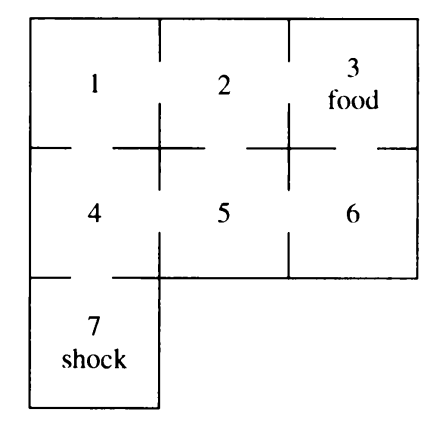
\includegraphics[width=0.3\textwidth]{Q345}
  \end{center}
  It moves through the compartments at random; i.e., if there are $k$ ways to leave a compartment, it chooses each of these with probability $1/k$. What is the probability that it finds the food in compartment 3 before feeling the electric shock in compartment 7?

  \begin{proof}
    Let $X_n$ denote the compartment occupied at stage $n$. The appropriate transition probability matrix for the movement of the rat is
    \begin{center}
      $P$ = \begin{tabular}{c ||c c c c c c c||} \multicolumn{1}{c}{\phantom{A}} & \multicolumn{1}{c}{$1$} & \multicolumn{1}{c}{$2$} & \multicolumn{1}{c}{$3$} & \multicolumn{1}{c}{$4$} & \multicolumn{1}{c}{$5$} & \multicolumn{1}{c}{$6$} & \multicolumn{1}{c}{$7$}\\
        $1$ & $0$ & $\frac{1}{2}$ & $0$ & $\frac{1}{2}$ & $0$ & $0$ & $0$ \\
        $2$ & $\frac{1}{3}$ & $0$ & $\frac{1}{3}$ & $0$ & $\frac{1}{3}$ & $0$ & $0$ \\
        $3$ & $0$ & $0$ & $1$ & $0$ & $0$ & $0$ & $0$ \\
        $4$ & $\frac{1}{3}$ & $0$ & $0$ & $0$ & $\frac{1}{3}$ & $0$ & $\frac{1}{3}$ \\
        $5$ & $0$ & $\frac{1}{3}$ & $0$ & $\frac{1}{3}$ & $0$ & $\frac{1}{3}$ & $0$ \\
        $6$ & $0$ & $0$ & $\frac{1}{2}$ & $0$ & $\frac{1}{2}$ & $0$ & $0$ \\
        $7$ & $0$ & $0$ & $0$ & $0$ & $0$ & $0$ & $1$ \\
      \end{tabular}.
    \end{center}
    Let $u_i$ denote the probability of absorption in the food compartment 3, given that the rat is dropped initially in compartment $i$. Then,
    \[
      U = \begin{bmatrix}
        u_1 \\
        u_2 \\
        u_4 \\
        u_5 \\
        u_6
      \end{bmatrix} = \begin{bmatrix}
        0 & \frac{1}{2} & \frac{1}{2} & 0 & 0 \\
        \frac{1}{3} & 0 & 0 & \frac{1}{3} & 0 \\
        \frac{1}{3} & 0 & 0 & \frac{1}{3} & 0 \\
        0 & \frac{1}{3} & \frac{1}{3} & 0 & \frac{1}{3} \\
        0 & 0 & 0 & \frac{1}{2} & 0 \\
      \end{bmatrix}U + \begin{bmatrix}
        0 \\
        \frac{1}{3} \\
        0 \\
        0 \\
        \frac{1}{2}
      \end{bmatrix},
    \]
    and the linear system yields
    \[
      U = \begin{bmatrix}
        1 & -\frac{1}{2} & -\frac{1}{2} & 0 & 0 \\
        -\frac{1}{3} & 1 & 0 & -\frac{1}{3} & 0 \\
        -\frac{1}{3} & 0 & 1 & -\frac{1}{3} & 0 \\
        0 & -\frac{1}{3} & -\frac{1}{3} & 1 & -\frac{1}{3} \\
        0 & 0 & 0 & -\frac{1}{2} & 1 \\
      \end{bmatrix}^{-1}\begin{bmatrix}
        0 \\
        \frac{1}{3} \\
        0 \\
        0 \\
        \frac{1}{2}
      \end{bmatrix} = \begin{bmatrix}
        \frac{7}{12} \\
        \frac{3}{4} \\
        \frac{5}{12} \\
        \frac{2}{3} \\
        \frac{5}{6}
      \end{bmatrix}.
    \]
    It follows that $u_4 = \frac{5}{12}$.
  \end{proof}
\end{homeworkProblem}

\newpage

\begin{homeworkProblem}
  A baseball trading card that you have for sale may be quite valuable. Suppose that the successive bids $\xi_1, \xi_2, \ldots$ that you receive are independent random variables with the geometric distribution

  \[
    \Pr\{\xi = k\} = 0.01(0.99)^k \quad \text{for} \quad k = 0, 1, \ldots.
  \]

  If you decide to accept any bid over \$100, how many bids, on the average, will you receive before an acceptable bid appears?

  \begin{proof}
    The transition probability from $i$ bids to $j$ bids is
    \[
      P_{ij} = \begin{cases}
        \Pr\{\xi_j < 100\}, & j = i + 1 \\
        \Pr\{\xi_j \geq 100\}, & j = 0 \\
        0, & \text{otherwise}
      \end{cases} = \begin{cases}
        1 - (0.99)^{100}, & j = i + 1 \\
        (0.99)^{100}, & j = 0 \\
        0, & \text{otherwise}
      \end{cases}.
    \]
    Let $T = \inf\{n \geq 0; \xi_{n + 1} > 100\}$. Note that $\E[T|\xi_1 < 100] = \E[T] + 1$ and $\E[T|\xi_1 \geq 100] = 1$. Then,
    \begin{align*}
      \E[T]
      &= \E[T|\xi_1 \geq 100]P_{00} + \E[T|\xi_1 < 100]P_{01} \\
      &= P_{00} + (1 + \E[T])(1 - (0.99)^{100}) \\
      &= \frac{1}{(0.99)^{100}} \approx 2.73
    \end{align*}
  \end{proof}
\end{homeworkProblem}

\newpage

\begin{homeworkProblem}
  Martha has a fair die with the usual six sides. She throws the die and records the number. She throws the die again and adds the second number to the first. She repeats this until the cumulative sum of all the tosses first exceeds 10. What is the probability that she stops at a cumulative sum of 13?

  \begin{proof}
    Let $X_n$ denote the sum after $n$ attempts to throw. The transition probability matrix is
    \begin{center}
      $P$ = \begin{tabular}{c ||c c c c c c c c c c c c c||} \multicolumn{1}{c}{\phantom{A}} & \multicolumn{1}{c}{$0$} & \multicolumn{1}{c}{$1$} & \multicolumn{1}{c}{$2$} & \multicolumn{1}{c}{$3$} & \multicolumn{1}{c}{$4$} & \multicolumn{1}{c}{$5$} & \multicolumn{1}{c}{$6$} & \multicolumn{1}{c}{$7$} & \multicolumn{1}{c}{$8$} & \multicolumn{1}{c}{$9$} & \multicolumn{1}{c}{$10$} & \multicolumn{1}{c}{$13$} & \multicolumn{1}{c}{$X$} \\
        $0$ & $0$ & $\frac{1}{6}$ & $\frac{1}{6}$ & $\frac{1}{6}$ & $\frac{1}{6}$ & $\frac{1}{6}$ & $\frac{1}{6}$ & $0$ & $0$ & $0$  & $0$ & $0$ & $0$ \\
        $1$ & $0$ & $0$ & $\frac{1}{6}$ & $\frac{1}{6}$ & $\frac{1}{6}$ & $\frac{1}{6}$ & $\frac{1}{6}$ & $\frac{1}{6}$ & $0$ & $0$ & $0$  & $0$ & $0$ \\
        $2$ & $0$ & $0$ & $0$ & $\frac{1}{6}$ & $\frac{1}{6}$ & $\frac{1}{6}$ & $\frac{1}{6}$ & $\frac{1}{6}$ & $\frac{1}{6}$ & $0$ & $0$ & $0$  & $0$ \\
        $3$ & $0$ & $0$ & $0$ & $0$ & $\frac{1}{6}$ & $\frac{1}{6}$ & $\frac{1}{6}$ & $\frac{1}{6}$ & $\frac{1}{6}$ & $\frac{1}{6}$ & $0$ & $0$ & $0$ \\
        $4$ & $0$ & $0$ & $0$ & $0$ & $0$ & $\frac{1}{6}$ & $\frac{1}{6}$ & $\frac{1}{6}$ & $\frac{1}{6}$ & $\frac{1}{6}$ & $\frac{1}{6}$ & $0$ & $0$ \\
        $5$ & $0$ & $0$ & $0$ & $0$ & $0$ & $0$ & $\frac{1}{6}$ & $\frac{1}{6}$ & $\frac{1}{6}$ & $\frac{1}{6}$ & $\frac{1}{6}$ & $0$ & $\frac{1}{6}$ \\
        $6$ & $0$ & $0$ & $0$ & $0$ & $0$ & $0$ & $0$ & $\frac{1}{6}$ & $\frac{1}{6}$ & $\frac{1}{6}$ & $\frac{1}{6}$ & $0$ & $\frac{2}{6}$ \\
        $7$ & $0$ & $0$ & $0$ & $0$ & $0$ & $0$ & $0$ & $0$ & $\frac{1}{6}$ & $\frac{1}{6}$ & $\frac{1}{6}$ & $\frac{1}{6}$ & $\frac{2}{6}$ \\
        $8$ & $0$ & $0$ & $0$ & $0$ & $0$ & $0$ &  $0$ & $0$ & $0$ & $\frac{1}{6}$ & $\frac{1}{6}$ & $\frac{1}{6}$ & $\frac{3}{6}$ \\
        $9$ & $0$ & $0$ & $0$ & $0$ & $0$ & $0$ & $0$ & $0$ & $0$ & $0$ & $\frac{1}{6}$ & $\frac{1}{6}$ & $\frac{4}{6}$ \\
        $10$ & $0$ & $0$ & $0$ & $0$ & $0$ & $0$ & $0$ & $0$ & $0$ & $0$ & $0$ & $\frac{1}{6}$ & $\frac{5}{6}$ \\
        $13$ & $0$ & $0$ & $0$ & $0$ & $0$ & $0$ & $0$ & $0$ & $0$ & $0$ & $0$ & $1$ & $0$ \\
        $X$ & $0$ & $0$ & $0$ & $0$ & $0$ & $0$ & $0$ & $0$ & $0$ & $0$ & $0$ & $0$ & $1$ \\
      \end{tabular}
    \end{center}
    Note that $(P^{(n)})_{ij} = \p(X_n = j|X_0 = i)$. Since we must end up with a sum greater than 10 after $11$ throws, $(P^{(11)})_{0, 13}$ is the probability of ending up at $13$. According to Matlab, $(P^{(11)})_{0, 13} \approx 0.1819$.
  \end{proof}
\end{homeworkProblem}

\newpage

\begin{homeworkProblem}
  Suppose a parent has no offspring with probability $\frac{1}{2}$ and has two offspring with probability $\frac{1}{2}$. If a population of such individuals begins with a single parent and evolves as a branching process, determine $u_n$, the probability that the population is extinct by the $n$th generation, for $n = 1, 2, 3, 4, 5$.

  \begin{proof}
    Since 
    \[
      u_n = \frac{1}{2}[1 + (u_{n - 1})^2],
    \]
    \begin{gather*}
      u_1 = 0.5, \quad u_2 = 0.625, \quad u_3 = 0.695, \quad u_4 = 0.742, \quad u_5 = 0.775.
    \end{gather*}
  \end{proof}
\end{homeworkProblem}
\end{document}